% Give an overview of PUF devices

\chapter{Physically Unclonable Functions}
\label{chapter:pufoverview}
It is desirable for a user to be sure that the device that he is using is authentic. However, due to the sophistication
of forgeries or possible communication tampering, a user might be suspicious that the system is the system it claims
to be. A device called a Physically Unclonable Function, or PUF, is a technology that remedies this problem.

A PUF device provides a unique challenge-response capability. That is, when two PUFS are provided the identical
challenge, they will each produce unique responses. In this way, a PUF, and the system it contains, 
can be identified by the response value it generates to a specific challenge. A more formalized definition of
this relationship is given below.

\begin{align*}
PUF_1(C) = R_1\\
PUF_2(C) = R_2\\
R_1 \neq R_2
\end{align*}

\section{Types of PUFs}
A PUF device provides this sort of relationship by leveraging the physical properties
of the materials in which it is instantiated. There are several different ways of doing
this, from measuring the distortions of reflected light to leveraging the
manufacturing inconsistencies from one chip to another.

The Ring Oscillator PUF is presented first and in somewhat greater detail than
other types of PUF since this is the type of PUF that the author worked with primarily.
As such, it was incorporated in many of the different applications presented later in
Chapters ~\ref{chapter:rok}, ~\ref{chapter:pear}, and ~\ref{chapter:doe}.

\subsection{Ring Oscillator PUF}
A Ring Oscillator PUF is a PUF design that utilizes a circuit called a Ring 
Oscillator (RO). An RO is an odd number of inverter gates tied together. Because
there are an odd number of gates, this will produce a continuously changing,
or oscillating, signal. Because it is a combination of circuits, the RO PUF can
be instantiated on a piece of silicon, such as an FPGA or ASIC device.

\begin{figure}[!ht] % The h specifies to place the figure 'here' as in, inline with the source code
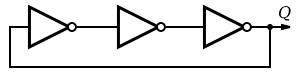
\includegraphics[]{images/ro.png}
\caption{A 3 gate Ring Oscillator}
\label{fig:ro}
\end{figure}
\FloatBarrier

Depending on the number of inverter gates being used
as well as the propagation delay of every individual inverter, the output
frequency of one RO may be different from another RO. In Figure ~\ref{fig:ro},
this output signal corresponds to the signal marked $Q$.

When used as part of a PUF, the unique behaviour of an RO will be examined.
Consider again the 3 stage RO as shown in Figure \ref{fig:ro}. All three
inverter gates are assumed to have the same propagation delay and the
interconnecting wires are assumed to impose a negligible delay. However, in
an actual instantiation of an RO, these assumptions are invalid. All three inverters
should have the same propagation delay, but, due to uncontrollable manufacturing
inconsistencies and tolerances, they do not. In a similar vein, the interconnecting
wires will also impose a non-zero delay time in signal propagation. Both of these
factors will combine so that even if two ROs are produced on the same 
manufacturing line, they will generate a slightly different output frequency.

The slightly different output frequencies of two ring oscillators forms the basis
of randomness for the Ring Oscillator PUF. Because the output frequencies of the
ROs cannot be predicted, their actual frequency at runtime gives a way to uniquely
identify the individual PUF that contains them. In Figure \ref{fig:ropuf}, a more
detailed diagram of a PUF based off of ring oscillators is presented.

\begin{figure}[ht!]
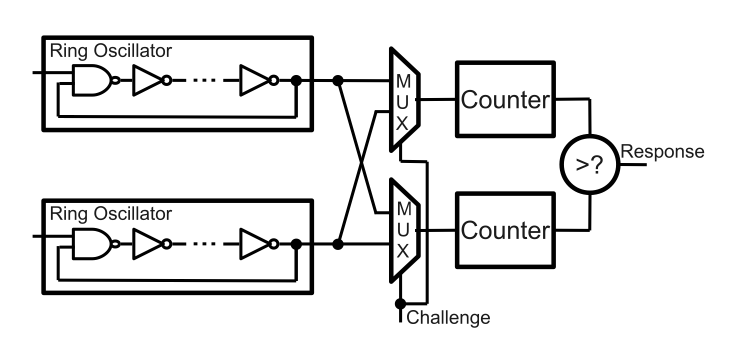
\includegraphics[width=500px]{images/ropuf.png}
\caption{A 1-bit Ring Oscillator PUF}
\label{fig:ropuf}
\end{figure}
\FloatBarrier

The ring oscillator PUF shown above uses a challenge bit and feeds it to a multiplexer.
If the challenge bit is zero, the top ring oscillator will be fed to the top counter and
the bottom ring oscillator to the bottom counter. If the challenge bit is one, the top
ring oscillator will be fed to the bottom counter and the bottom ring oscillator will
be fed to the top counter. The counters will then be executed for a given amount of time.
At the expiration of this time duration, the values of the counters are compared. If the
top counter has a larger total, a zero is output as the response. If the bottom counter
has a larger total, a one is output as the response. 
While the diagram only displays two ring oscillators and only 1 bit of challenge and
response, this diagram can be extrapolated to form arbitrarily large PUFs.

That is the most basic design of an RO PUF. In practice, this design is somewhat 
inefficient, since for an N-bit PUF, 2*N ring oscillators are needed, which is fairly
expensive. There has been work done for alternative designs of
an RO PUF to reduce the number of ring oscillators needed ~\cite{aegis_pool}. 
Typically, this involves using
a pool of ring oscillators and then using a multi-bit challenge to select some permutation
of them. Details presented in ~\cite{aegis_pool} illustrate that 35 oscillators can
be used to generate 133-bits of output by using this pool strategy.

\subsection{Butterfly PUF}
Another design of a PUF is called a Butterfly PUF. This design is similar to the previous
RO design in that it can be instantiated on a piece of silicon. This allows for easy
incorporation into existing FPGA designs or through the production of a custom ASIC chip.
Figure~\ref{fig:butterfly} shows a circuit example of a butterfly PUF and how it might be
designed.

The Butterfly PUF works by tying the output of two D flip flops to each other's inputs. By applying
the CLR signal to one flip flop and the PRE signal to the other flip flop, the circuit will enter an
undefined state. It will eventually go to one of two defined states (0 or 1). The circuit will typically
settle in the same state, which forms the basis for the PUF response.

Interested readers are referred to \cite{butterflypuf} for more information about the Butterfly PUF.

\begin{figure}[ht!]
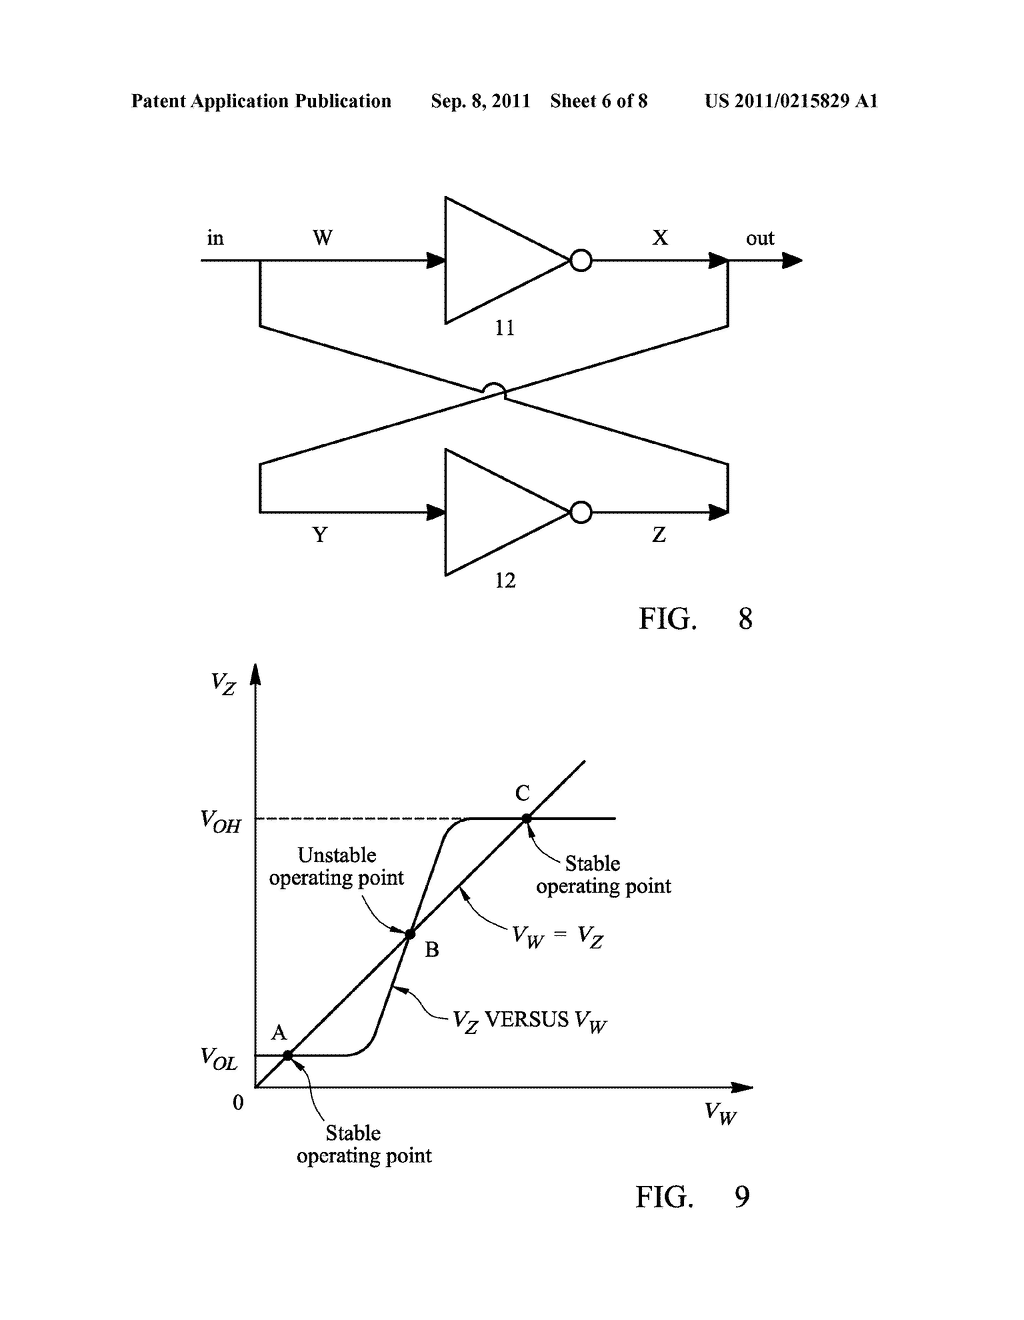
\includegraphics[scale=.70]{images/butterflypuf.png}
\caption{A depiction of a Butterfly PUF}
\label{fig:butterfly}
\end{figure}
\FloatBarrier

\subsection{Optical PUF}
An optical PUF is a design that leverages physical randomness that is explicitly introduced during
a manufacturing process. The typical optical PUF is constructed by taking a transparent material
and randomly coating it with particles to disperse the light. A laser light is then shone on the material
and the resulting pattern is recorded. The image is then processed and this is the response of the
PUF. Interested readers are referred to the original thesis that proposed this idea in \cite{opticalpuf}.

\subsection{Coating PUF}
A coating PUF works by creating a mesh of wires and then filling the cavities with some sort of
dielectric material. Based on how the dielectric is applied, there will be varying levels of capacitance
between the wires in the mesh. This capacitance can then be measured as the unique response for
the given PUF design. Details are presented in \cite{coatingpuf}. 

The coating PUF is typically used as a sort of anti-tamper device. The coating PUF is wrapped
around an existing circuit and is used to enable its operation. That is, the proper PUF response
is needed to unlock the device. If an adversary is to alter the coating in anyway (though reverse engineering 
for example), this will alter the PUF response and cause the underlying circuit to not function. 

\section{PUF Error and Error Correction}
An important part to consider for any PUF device is the stability of its output for
the same input. If the PUF device yields different outputs for the same challenge, the
utility of a PUF is greatly reduced. As such, it is important to examine and investigate
the stability and error rates of PUF. As the author worked primarily with RO PUFs, unless
otherwise noted, this section refers to RO PUFs.

The basic use case that should be examined is when a PUF is executed twice in the same
environment; that is, temperature, humidty, and other environmental factors are constant.
For the RO PUF design in Figure \ref{fig:ropuf}, error rates can be reduced by increasing
the time that the ring oscillators are executed. In this way, the faster ring oscillator's
counter will clearly dominate the slower ring oscillator's counter. If the execution time
is very brief, start-up times and routing delays may impose a noticeable difference and
induce additional error. Note that when the author refers to increasing timer execution
time, he is discussing orders of milliseconds. The ring oscillators were typically run
at upwards of 100 MHz, so several milliseconds was enough time for frequency differences
to become apparent.

% temperature
A source of error that can be introduced is a change in temperature. Circuits will run 
either faster or slower as temperature changes, due to the changing resistance of the
internal components. Note that this is not a behaviour specific to PUFs, but electronics
in general. As such, it is important to consider the effect of temperature on PUF devices.
Work in ~\cite{puftemp} presents detailed, empirical studies of temperature's effect on
PUFs.

% supply voltage variation

% aging
Circuit aging is another source of error that can potentially affect PUFs. Over time,
certain pathways and routes of the PUF may change in their propagation delay. Since the
PUF is predicated upon the same routes being used over and over, this can cause drastic
problems for the PUF. At the least, aging can make a PUF more susceptible to other
sources of error, but at worst case, it could cause enough bits of the PUF to change
from their original values so that the PUF is no longer identifiable as the original PUF.
Interested readers are referred to work in ~\cite{pufaging} 
which discusses PUF aging in greater detail.

% Discuss typical PUF error hamming distance

\subsection{Error Correction}
As previously described, there are multiple different factors that can affect PUFs
and their execution. If these are not mitigated, the functionality and utility of a PUF
is greatly reduced. As such, an error correction scheme is typically needed when employing
a PUF device.

Usually, the raw PUF response is not directly output, but rather, is fed into an
error correction block. The error correction block processes the raw PUF output and
removes any small errors that may be apparent and outputs the corrected response.
This is diagrammed in Figure \ref{fig:pufecc}. While it is possible to do the error
correction on a discrete chip separate from the PUF itself, it is safer to perform the
error correction on the same chip as the PUF. This prevents an adversary from potentially
intercepting the raw PUF output as it is transmitted to the error correction block. Note
that in Figure \ref{fig:pufecc}, there is a notation that the PUF and the error correction
are self contained to illustrate this.

\begin{figure}[!ht]
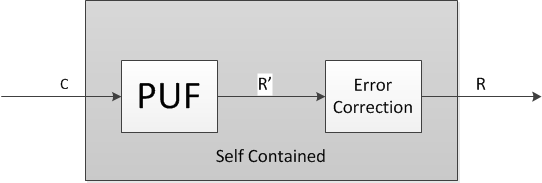
\includegraphics[]{images/puf_ecc.png}
\caption{A high level concept of PUF error correction}
\label{fig:pufecc}
\end{figure}

The author has typically employed the use of Reed-Solomon (RS) error correction codes to do 
error correction. By adding $t$ RS symbols, up to $t$ bit errors can be detected, 
while $t/2$ bit errors can actually be corrected. This is a fairly large amount of
errors to correct. For a ring oscillator PUF, \cite{pufhammingdistance} found that inter-chip
variation (that is, the same challenge) in response was approximately 0.86\%. For a 128 bit PUF,
that equates to around 1 bit of error per execution. As such, not a lot of error correction is needed,
but some is indeed needed. In the author's work \cite{PEAR} \cite{PUFROK} \cite{CODASPY}, he has typically 
used 32 bits of Reed-Solomon error codes. This allows for detection of up to 32 bit errors 
in the 128 bits and correct up to 16 bit errors, which is usually sufficient.

\section{Vulnerabilities}
Besides just correcting for benign errors due to the nature of PUFs, it is important to consider
malicious tampering and how vulnerable the PUF is. Again, the use of PUF in this section refers
to the ring oscillator design previously described unless otherwise noted.

% Differential power analysis (security engineering, chapter 15)
There is a class of attacks called differential power analysis, \textit{DPA}, that needs to be considered
for PUFs. This involves monitoring the power consumption of a circuit during its execution. It is then possible
to deduce what bits of data are being processed at a given time. For example, if the floating point processor
takes a considerable amount of power in a microcontroller, an attacker could monitor the power during execution.
When he saw the power usage spike, he could infer that a floating point operation was taking place. This attack
is detailed in several papers and a fairly good overview is given in the book \cite{securityengineering}.

The ring oscillator PUF design is fairly resilient against this type of attack however. During execution of the
PUF, every ring oscillator will be executing simultaneously as well as the other support circuitry. Because
every execution utilizes the ring oscillators, power consumption will be constant. This thus eliminates the
power differences needed for DPA.

% Tampering
Tampering with the PUF itself is a vulnerability that needs to be considered. An attacker may attempt
to reverse engineer the PUF so that he could model and impersonate it. This would involve measuring
the distances between wires, capacitances, and propagation delays of the various elements of the PUF.
However, these elements are so small (nanometers) that the invasive techniques for measuring them
would likely alter their qualities, so any measurements taken would not be usable for impersonating
the original PUF. As such, tampering can destroy a PUF and its usability, but the risk of being able
to duplicate and impersonate the PUF is very very low.

% Supply chain corruption
Another important aspect that needs to be considered is if the PUF is tampered with at any point
during the manufacturing or delivery process. The main concern is that an attacker could intercept
the PUF and create a model of it; that is, the response for every possible challenge. It is possible to
offset this risk however by using sufficiently large PUFs. If a 128 bit PUF is used, this sort of attack
would require storing $2^{128}$ different values. There are estimated to be about $2^80$ atoms
in the universe so this attack is not very realistic.

\section{Comparison to Alternatives}
Several technologies exist that fulfill roles similar to the of PUF technology. The Trusted Platform Module (TPM)
and Radio Frequency Identification Tags (RFID Tags) are described below, as these are two very common
technologies that are in practice today.

\subsection{Trusted Platform Module}
Trusted Platform Modules (TPM) are a technology that is similar, but different than PUFs. They are
typically integrated into a computer's motherboard, though they are also present in other applications.

TPMs typically provide a large variety of services, as they are technically a cryptoprocessor. This is in
contrast to a PUF device, which is just a provider of the challenge-response capability. TPMs are used
to provide remote attestation, binding, and data sealing. These services leverage an \textit{endorsement 
key}, which is installed in the TPM at manufacture time.

One area where TPMs and PUFs differ is that TPMs only have their one secret endorsement key to act
as the key to all operations. If this is ever compromised, such as when it is being burned in at
manufacturing time, all TPM security is lost. In contrast, PUFs behaviour is characteristic of the challenge
provided. If a sufficiently large key space is chosen, such as 128 bits, then it is unrealistic that an
attacker could ever model the entire response space, which would encompass $2^{128}$ possible choices.

Readers interested in more about TPMs are referred to the TPM standards in~\cite{tpm}.

\subsection{Radio Frequency Identification Tags}
Radio Frequency Identification Tags, or RFID, are devices that are exposed to radio waves, which then
allow a reader device to read the information stored on the tag. They sometimes do not require power
and can operate off the power from the reader itself.

The information stored on tags is typically personally identifiable information, such as ID numbers,
location of origin, or related data. RFID tags are used in applications such as livestock inventory,
shipping containers, or warehouse progress.

A security concern with RFID tags is that they can be read passively and silently by unintended persons.
For instance, someone might carry a reader in his pocket and record the data about people walking
by him. This is a security risk and there has been some controversy over it.

RFID tags are a contrast to PUF. RFID tags simply store data and reads it out when queried. In contrast,
PUFs are a function that requires a specific input to get the desired response. In this way, more security
is present.
